\begin{figure}[h]
\centering
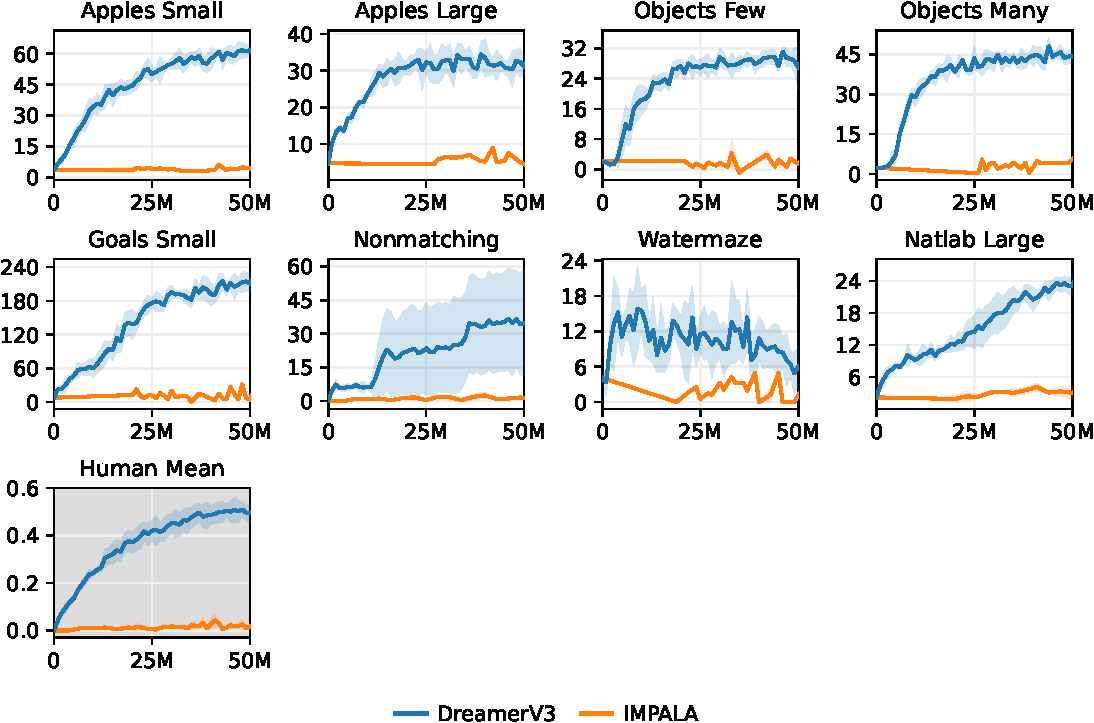
\includegraphics[width=1\linewidth]{dmlab/dmlab}
\caption{DMLab scores with a budget of 50M frames. Separate agents were trained for each task, corresponding to the IMPALA Experts method in \citet{espeholt2018impala}. Data efficiency is not the goal of IMPALA and it might be possible to tune it for improved data efficiency. Longer training curves and asymptotic performance of IMPALA are included in \cref{sec:dmlab_eff}.}
\label{fig:dmlab}
\end{figure}

\section*{Results}
\label{sec:experiments}

We perform an extensive empirical study to evaluate the generality and scalability of DreamerV3 across diverse domains---with over 150 tasks---under fixed hyperparameters.
We designed the experiments to compare DreamerV3 to the best methods in the literature, which are often specifically designed to the benchmark at hand.
Moreover, we apply DreamerV3 to the challenging video game Minecraft.
\Cref{tab:benchmarks} gives an overview of the domains.
For DreamerV3, we directly report the performance of the stochastic training policy and avoid separate evaluation runs using the deterministic policy, simplifying the setup.
All DreamerV3 agents are trained on one Nvidia V100 GPU each, making the algorithm widely usable across research labs.
The source code and numerical results are available on the project website:
\url{https://danijar.com/dreamerv3}

\pagebreak  % TODO

\paragraph{Benchmarks}
To evaluate the generality of DreamerV3, we perform an extensive empirical evaluation across 7 domains that include continuous and discrete actions, visual and low-dimensional inputs, dense and sparse rewards, different reward scales, 2D and 3D worlds, and procedural generation.
\Cref{fig:summary} summarizes the results, with training curves and score tables included in the appendix.
DreamerV3 achieves strong performance on all domains and outperforms all previous algorithms on 4 of them, while also using fixed hyperparameters across all benchmarks.
\begin{itemize}
\itempar{Proprio Control Suite} This benchmark contains 18 continuous control tasks with low-dimensional inputs and a budget of 500K environment steps \citep{tassa2018dmcontrol}. The tasks range from classical control over locomotion to robot manipulation tasks. DreamerV3 sets a new state-of-the-art on this benchmark, outperforming D4PG \citep{barth2018d4pg}, DMPO \citep{abdolmaleki2020dmpo}, and MPO \citep{abdolmaleki2018mpo}.
\itempar{Visual Control Suite} This benchmark consists of 20 continuous control tasks where the agent receives only high-dimensional images as inputs and a budget of 1M environment steps \citep{tassa2018dmcontrol,hafner2020dreamerv2}. DreamerV3 establishes a new state-of-the-art on this benchmark, outperforming DrQ-v2 \citep{yarats2021drqv2} and CURL \citep{srinivas2020curl} which additionally require data augmentations.
\itempar{Atari 100k} This benchmark includes 26 Atari games and a budget of only 400K environment steps, amounting to 100K steps after action repeat or 2 hours of real time \citep{kaiser2019simple}. EfficientZero \citep{ye2021effzero} holds the state-of-the-art on this benchmark by combining online tree search, prioritized replay, hyperparameter scheduling, and allowing early resets of the games; see \cref{tab:atari100k_setting} for an overview. Without this complexity, DreamerV3 outperforms the remaining previous methods such as the transformer-based IRIS \citep{micheli2022iris}, the model-free SPR \citep{schwarzer2020spr}, and SimPLe \citep{kaiser2019simple}.
\itempar{Atari 200M} This popular benchmark includes 55 Atari video games with simple graphics and a budget of 200M environment steps \citep{bellemare2013ale}. We use the sticky action setting \citep{machado2018revisiting}. DreamerV3 outperforms DreamerV2 with a median score of 302\% compared to 219\%, as well as the top model-free algorithms Rainbow \citep{hessel2018rainbow} and IQN \citep{dabney2018iqn} that were specifically designed for the Atari benchmark.
\itempar{BSuite} This benchmark includes 23 environments with a total of 468 configurations that are designed to test credit assignment, robustness to reward scale and stochasticity, memory, generalization, and exploration \citep{osband2019bsuite}. DreamerV3 establishes a new state-of-the-art on this benchmark, outperforming Bootstrap DQN \citep{osband2016bootdqn} as well as Muesli \citep{hessel2021muesli} with comparable amount of training. DreamerV3 improves over previous algorithms the most in the credit assignment category.
\itempar{Crafter} This procedurally generated survival environment with top-down graphics and discrete actions is designed to evaluate a broad range of agent abilities, including wide and deep exploration, long-term reasoning and credit assignment, and generalization \citep{hafner2021crafter}. DreamerV3 sets a new state-of-the-art on this benchmark, outperforming PPO with the LSTM-SPCNN architecture \citep{stanic2022crafterobject}, the object-centric OC-SA \citep{stanic2022crafterobject}, DreamerV2 \citep{hafner2020dreamerv2}, and Rainbow \citep{hessel2018rainbow}.
\item
\parbox[t]{\dimexpr\textwidth-\leftmargin}{%
\vspace{-2.5mm}
\begin{figure}[h]
\centering
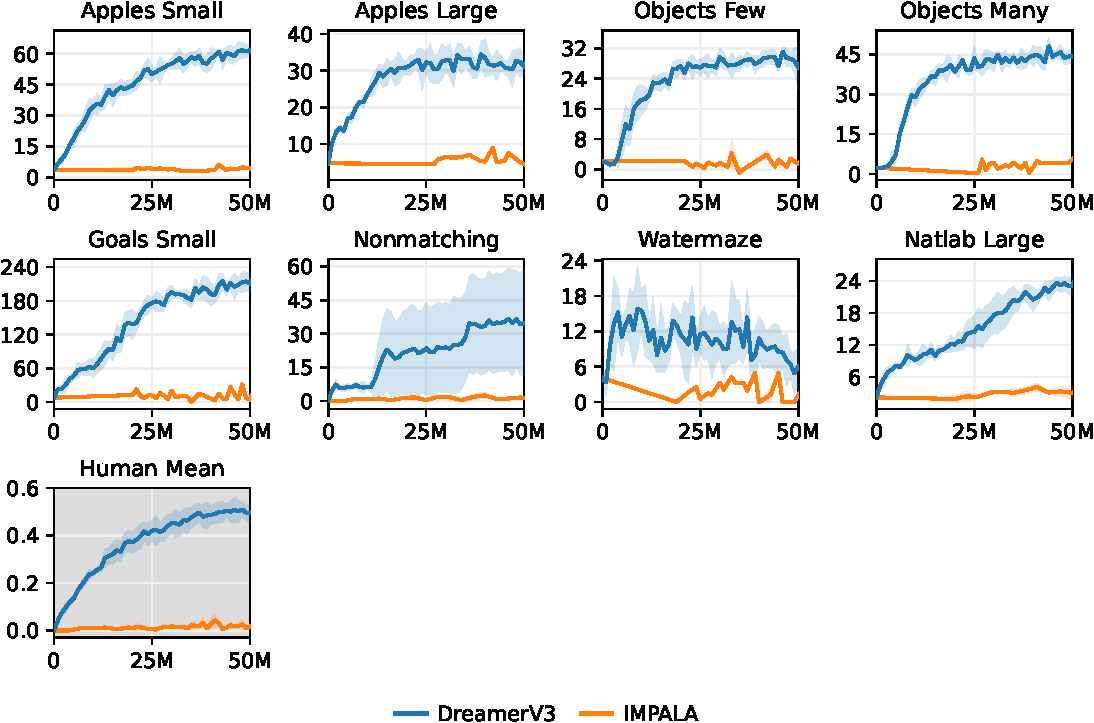
\includegraphics[width=1\linewidth]{dmlab/dmlab}
\caption{DMLab scores with a budget of 50M frames. Separate agents were trained for each task, corresponding to the IMPALA Experts method in \citet{espeholt2018impala}. Data efficiency is not the goal of IMPALA and it might be possible to tune it for improved data efficiency. Longer training curves and asymptotic performance of IMPALA are included in \cref{sec:dmlab_eff}.}
\label{fig:dmlab}
\end{figure}
\textbf{DMLab}\quad This domain contains 3D environments that require spatial and temporal reasoning \citep{beattie2016dmlab}. On 8 challenging tasks, DreamerV3 matches and exceeds the final performance on the scalable IMPALA agent \citep{espeholt2018impala} in only 50M compared to 10B environment steps, amounting to a data-efficiency gain of over 13000\%. We note that IMPALA was not designed for data-efficiency but serves as a valuable baseline for the performance achievable by scalable RL algorithms without data constraints.}
\end{itemize}

\paragraph{Scaling properties}

Solving challenging tasks out of the box not only requires an algorithm that succeeds without adjusting hyperparameters, but also the ability to leverage large models to solve hard tasks.
To investigate the scaling properties of DreamerV3, we train 5 model sizes ranging from 8M to 200M parameters.
As shown in \Cref{fig:scaling}, we discover favorable scaling properties where increasing the model size directly translates to both higher final performance and data-efficiency.
Increasing the number of gradient steps further reduces the number of interactions needed to learn successful behaviors.
These insights serve as practical guidance for applying DreamerV3 to new tasks and demonstrate the robustness and scalability of the algorithm.

\paragraph{Minecraft}

Collecting diamonds in the open-world game Minecraft has been a long-standing challenge in artificial intelligence.
Every episode in this game is set in a different procedurally generated 3D world, where the player needs to discover a sequence of 12 milestones with sparse rewards by foraging for resources and using them to craft tools.
The environment is detailed in \cref{sec:mcenv}.
We following prior work \citep{kanitscheider2021minecraftcurriculum} and increase the speed at which blocks break because a stochastic policy is unlikely to sample the same action often enough in a row to break blocks without regressing its progress by sampling a different action.

Because of the training time in this complex domain, tuning algorithms specifically for Minecraft would be difficult.
Instead, we apply DreamerV3 out of the box with its default hyperparameters.
As shown in \cref{fig:summary}, DreamerV3 is the first algorithm to collect diamonds in Minecraft from scratch without using human data that was required by VPT \citep{baker2022vpt}.
Across 40 seeds trained for 100M environment steps, DreamerV3 collects diamonds in 50 episode.
It collects the first diamond after 29M steps and the frequency increases as training progresses.
A total of 24 of the 40 seeds collect at least one diamond and the most successful agent collects diamonds in 6 episodes.
The success rates for all 12 milestones are shown in \cref{fig:mcitems}.
